\documentclass{article}

\usepackage{graphicx}
\usepackage{txfonts}
\usepackage{subfigure}
\usepackage{epstopdf}
\usepackage{lineno}
\usepackage[authoryear,round]{natbib}
\usepackage[backref]{hyperref}
\usepackage{url}
\usepackage[inline]{enumitem}
\usepackage{verbatim}
\usepackage{csquotes}

\usepackage[authoryear,round]{natbib}
\usepackage[backref]{hyperref}
\usepackage{url}
%%    This version assumes using bibtex with the swsc bibliography style file
\bibliographystyle{swsc.bst}

\begin{document}
\title{Manuscript Ref: swsc160029}
\maketitle

\section*{Response to referees}
We thank the referees for their valuable feedback and critical assessment which helped to improve the quality of the article. We have revised the manuscript accordingly. In the following, the referees' comments are in italics, and our replies in normal text.\\

\textbf{Referee \#6}
\begin{enumerate}
\item \emph{Was the size of the training set of N=250 hourly values of Dst for the GP-AR model (and, additionally, V, Bz, VBz for the GP-ARX model) limited by the numerical effort to perform the matrix inversion? If yes, what resources did the inversion require?}

It is certainly true that Gaussian Process models become prohibitively expensive for very large training sets. Their computational complexity scales as $O(N^3)$, and this was commented in the manuscript on lines $161-165$.
However, a size of 250 is still very much below the computational limits of the method and, in our case, it has been decided by studying the performance of the models for increasing training sets. We have noticed that using sets with more than 250 values does not increase the overall performance.

We have made this point explicit on lines...

\item \emph{Both the training and model selection data sets did not include strong geomagnetic storms (Dst was between -30 and +37 in the training set and in a similar range in the model selection set).
What were the reasons for selecting these time periods in 2008 and 2014.
Why wasn't a stronger storm event included in the training or the model selection samples?
What justifies applying the models to stronger storms (the example shown in Figures 6 and 7 has Dst values down to -289nT)?} 

Additions were made in lines $229-234$ \blockquote{Although the training and model selection data sets both do not have a geomagnetic storm in them, this would not degrade the performance of \emph{GP-AR} and \emph{GP-ARX} because the linear polynomial kernel describes a non stationary and self similar Gaussian Process. This implies that for two events where the time histories of $Dst$, $V$ and $B_z$ are not close to each other but can be expressed as a diagonal rescaling of time histories observed in the training data, the predictive distribution is a linearly rescaled version of the training data $Dst$ distribution.}

\item \emph{The time lag parameters 'p' for the two models were selected by comparing the model to the 63 storm events. Shouldn't the parameter have been selected using an independent set of storms instead in order not to favor these new models against the other models?}

Additions were made in lines $242-247$ in section 4. \blockquote{The time lags chosen for \emph{GP-AR} are $p = 6$ while for \emph{GP-ARX} $p=6$, $p_{ex} = 1$. These vales have been decided by experimenting with values starting from one and choosing the value of $p$ yielding best performance on the 63 events in the bench mark. We do not feel that this approach for choosing the time lags leads to bias towards models which only perform well on the data set of \cite{Ji2012} because Gaussian Processes are not easily susceptible to overfitting for situations when the number of model hyper-parameters is small or leave one out cross-validation is not performed.}

\item \emph{Rastaetter et al. please correct the first initial in "A. Glocer".} 

Corrections made in lines $437-439$

\end{enumerate}
\textbf{Referee \#9}: 

\begin{enumerate}
\item \emph{In comparing their models with the existing six models, the authors claim that all these models are ONE STEP AHEAD models (Line 374 of the manuscript). They quote the results of Ji et al., (2012) for comparison. But when Ji et al. compared the six models, they did not run the six models in real OSA approach. As stated in Ji et al., (2012),  'When run the Dst model program for calculating the prediction value of Dst, we do not use the observed Dst data. We use the only previously predicted Dst data.' This means that all the six models take solar wind parameters exclusively as inputs. Thus their verification results for the six models are not in real ONE-STEP-AHEAD approach. The time advance of their predictions relies on the solar wind observation (or forecast). Such comparison is not convincing, and it is inappropriate to conclude that the new models are superior than all the existing models.}

We believe that the referee has misinterpreted the sentence quoted from Ji et al. (2012), and that all of the six models in that paper are indeed run as one-step-ahead models. Our interpretation of that statement is that it refers only to the TL model. That is the only model that indeed does not use the observed DST data as input. It uses some quantities, called $dst*$, that are calculated and advanced in time, by using observed solar wind quantities only. 
However, we agree that that statement is confusing and that it could lead to the referee's interpretation. We present two strong counter-arguments that should settle the issue.

The first argument is that we do not see any reason or benefit for comparing the models in the way the referee suggests they were compared, that is using the predicted $Dst$ values instead of the real and available $Dst$ data. It is obvious that by doing so the performance of the models would degrade, in ways that are difficult to foresee. The main and only purpose of the Ji et al. paper, however, is to compare the performance of different models. Why would one like to compare less-than-optimal results? That paper would be completely flawed if the authors had made what the referee suggests. 

We realize that the first argument is simply based on scientific common sense, and that the referee might not be persuaded. The following is a more scientific and indisputable proof that the referee's suggestion is wrong.
In the Ji et al. paper, NARMAX and TL are the most performing models. Since the referee's suggestion is irrelevant for TL (because it does not use $Dst$ by construction), we have tested it on NARMAX.
We have taken the NARMAX model as specified in Boynton et al. (2011) and re-tested it on the 63 storms, by using the previously predicted $Dst$ values instead of the actual $Dst$ data. This model is denoted as \emph{NM Variant} in
Figures \ref{fig:rmseNew} and \ref{fig:ccNew}. Here, we show the Root Mean Square Error and the Correlation Coefficient (same as Figure 2b and 2a in Ji et al. (2012)). By using predicted $Dst$, the RMSE changes from 23.4 to 54.8 and the CC goes from 0.87 to 0.04 (which means no-correlation). 
Clearly, the values reported in that paper could not have been obtained in the way the referee suggests. 

As a final remark to the comment \emph{all the six models take solar wind parameters exclusively as inputs}, and the fact that TL indeed does not use $DST$ as input, we reckon that comparisons should not only be made on models that input the same input parameters. Space weather users care only about the accuracy of the model’s prediction, regardless of what parameters the model inputs. Comparisons are fair as long as the same amount of information is potentially available to all models. However, it is a model designer choice which information to use and which to disregard.

\begin{figure}[h]
   \centering
   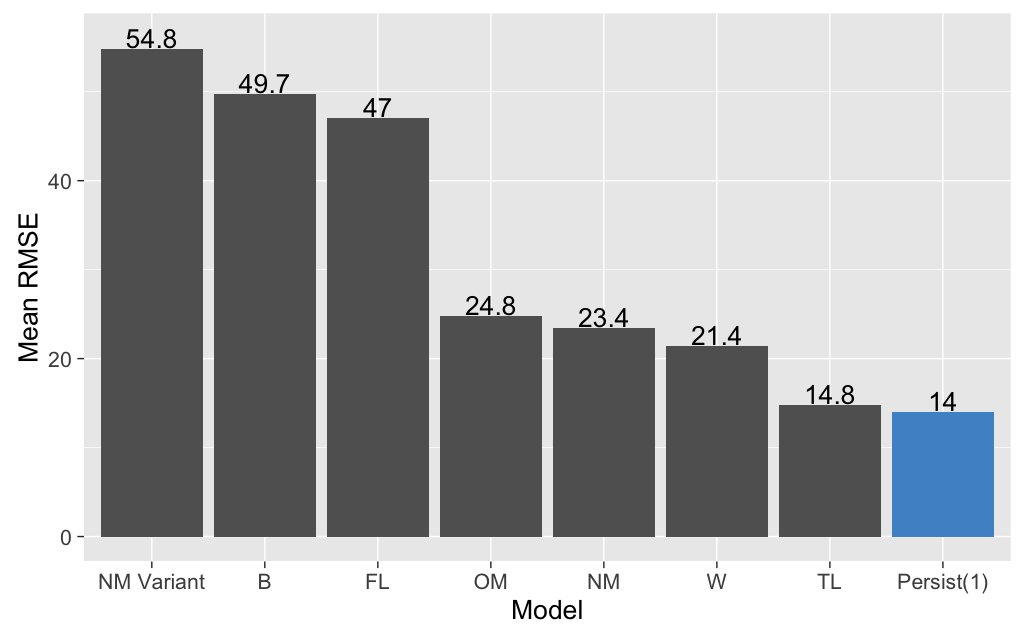
\includegraphics[width=\textwidth]{Compare_RMSE_New.png}
      \caption{
      Averaged RMSE performance of \emph{NARMAX Variant} and the 
      \emph{Persistence} model versus results in \cite{Ji2012}.
      }
      \label{fig:rmseNew}
\end{figure}

\begin{figure}
   \centering
   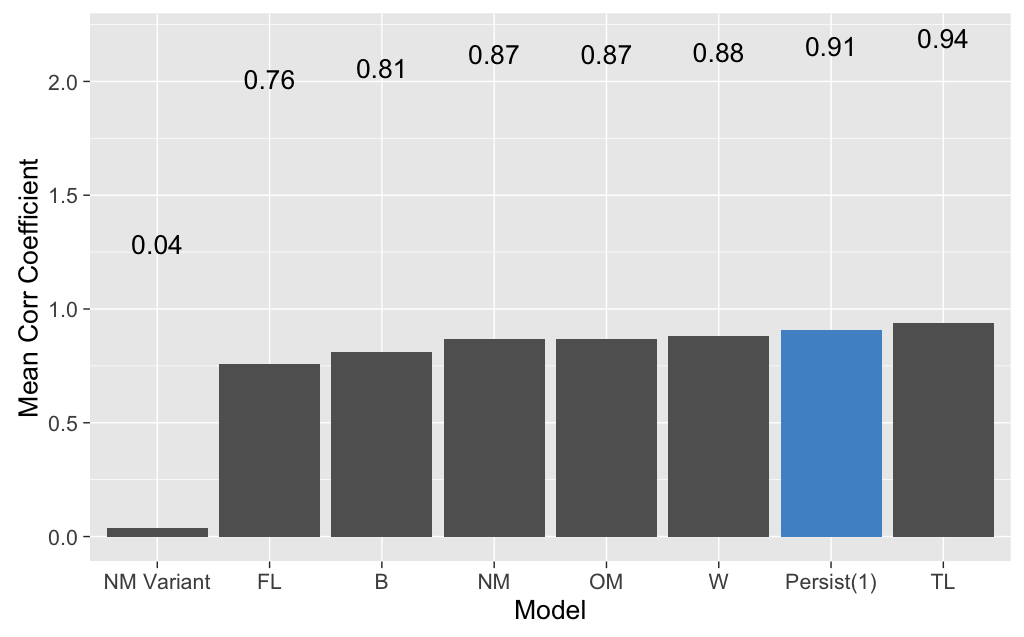
\includegraphics[width=\textwidth]{Compare_CC_New.png}
      \caption{Averaged cross correlation performance of \emph{NARMAX Variant} and the 
      \emph{Persistence} model versus results in \citet{Ji2012}.}
         \label{fig:ccNew}
\end{figure}

\item \emph{We know that Dst data are published by WDC Kyoto. The baseline for the Kyoto Dst is determined by measurements made during statistically quiet days. This results in a sequence of adjustments from “Quicklook” Dst values to “Provisional” (several years delay) and eventually “Final” values (after about 5 years) as the quiet days are determined by hindsight. By checking the WDC kyoto website it can be found that currently final data are available for years before 2011, provisional data for years 2012-2014, and Quicklook Dst after 2015. From literatures it was reported that there were large differences between provisional and final Dst (bigger than average error of some of the existing Dst models). Given this, when applied to real time operations, OSA models utilizing history of observed Dst (thus the Quicklook Dst) as input may introduce large errors. This may be one reason that existing Dst models utilize only solar wind data as input.}

First, it is not true that existing $Dst$ models utilize only solar wind data as input. NARMAX (one of the best performing model) uses the time history of $Dst$. Furthermore, since the differences among final, quicklook, and provisional $Dst$ are the quite days base line values, this does not affect the timing of the storms, but only the magnitude due to the subtraction of different offsets. Also, this would not change the evaluation of delta $Dst$, CC, RMSE, etc., provided that we consistently use the same type of Dst (e.g, we use only provisional or quicklook $Dst$s).
 
\item \emph{To test the strengths of the Gaussian Processes in predictive modeling, it is FINE to evaluate the model by taking FINAL Dst as input, as the authors did. But in comparing them with existing models to test the strength of a new modeling approach compared with other methods, all these models should be run in the same way (whether or not to input observed Dst). Once the new models outperform existing models when they are run in the same way, we can say that Gaussian Processes show stronger potential in predictive modeling.}

Unless we misunderstand the referee's comments, this is a repetition of point 1. 
\end{enumerate}


\bibliography{swsc}


\end{document}